% Document settings
\documentclass[11pt]{article}
\usepackage{fancyhdr}
\usepackage[margin=1in]{geometry}
\usepackage[pdftex]{graphicx}
\usepackage{multirow}
\usepackage{setspace}
\pagestyle{plain}
\usepackage[american voltages]{circuitikz}
%\usepackage[american]{circuitikz}
\usepackage{graphicx}
\usepackage{multirow}
\usepackage{booktabs}
\usepackage{epstopdf}
%\usepackage{MnSymbol,wasysym}
\usepackage{amsmath}
%\usepackage{mathtools}
\usepackage{amssymb}
\usepackage{lipsum}
\usepackage{sympytex}
\usepackage{siunitx}
\setlength\parindent{0pt}
\graphicspath{{images/}{drawings/}}
% % % % % % % % % % % Header footer
% % % % % % % % % % %EDIT THIS % % % % % % % % % % % % % % % % % % % %
\pagestyle{fancy}
\fancyhf{}
\lhead{Tech Memo:  Experiment 1-Voltage Division}
\rhead{Andrei Tumbar}
\lfoot{EE281}
\cfoot{02/04/2020}
\rfoot{Page \thepage}
% % % % % % % % % % % % % % % % % % % % % % % % % % % % % % % % % % % % %


\begin{document}
	\numberwithin{equation}{subsection}
	\numberwithin{figure}{subsection}
	\hspace{6in}
		
\includegraphics[scale=0.9,trim=0cm 0in 0in 0.0in,clip]{RIT_KGCOE1}
\newline

\Huge \textbf{EEEE 281: Experiment 1 \\Voltage Division}\\

\Large
\textbf{From:} Andrei Tumbar [Computer Engineering] \\
\textbf{To: } Section 2 TA: [edit] \\
\textbf{Date: } Performed: 02/04/2020  Due: 02/11/2020 \\
\textbf{Subject: } Lab 1\\
\textbf{Lab Partner(s): } N/A\\
\vspace{0.5in}
	\begin{table}[h!]
		\centering
%		\caption{Grading Table}
		\label{Table:Grading Table 1}
		%\begin{tabular}{llllll}
		\begin{tabular}{|c||c|c|c|c|}
			\hline
			Component & Percentage of Grade   & Score \hspace{0.25in} & Comment \hspace{1in}  \\
			\hline
			Report Formatting & 20~\si{\percent} & & \\	 
			\hline 
			Hand Calculations: Circuit 1 & 10~\si{\percent} & & \\
			%Hand Calculations: Circuit 2 & 5~\si{\percent} & & \\
			\hline	
			PSPICE Setup: & 5~\si{\si{\percent}}&&\\
			\hline
			PSPICE Simulation:  & 10~\si{\percent} & & \\
			\hline
			PSPICE Discussion:  & 10~\si{\percent} & & \\
			%PSPICE Simulation: Circuit 2 & 10~\si{\percent} & & \\
			\hline
			Experimental Setup: & 5~\si{\percent} & & \\
			\hline
		    Experimental Data:  & 20~\si{\percent} & & \\	
		    %Experimental Data: Circuit 2 & 10~\si{\percent} & & \\	 
			\hline
			Experimental Discussion:  & 20~\si{\percent} & & \\	 
			\hline
			\textbf{Total Score:}&  & & \\	 
			\hline
			\textbf{Graded By:}&  & & \\	 
			\hline
			
		\end{tabular}
	\end{table}
\newpage
\Large \textbf{Abstract} \\
\normalsize
In the first part of this exercise, the software portion, a circuit with three resistors (two 5.6 k\si{\ohm}, 1 k\si{\ohm}) in series was designed in PSPICE, a circuit design, and simulation program. The resistors were listed with tolerances. A simulation was run to display a histogram of likely outcomes given the tolerance and resistance rating of each resistor. A Monte Carlo simulation displayed a statistical analysis of the likely outcomes of testing the circuit. In the hardware portion of the exercise, the circuit was implemented on a breadboard. The voltage was measured across each resistor given a supplied voltage of 5V. An effective resistance was measured along with resistance from each resistor. Finally, the voltage of each node relative to ground was measured and recorded. These experimentally determined values were compared to those calculated using the voltage division laws to analyze the circuit.

\section {Introduction and Theory}

Write a paragraph to describe the objectives of the laboratory.  After this, follow the section headings in the template, including the required figures.

\subsection{Theory: Circuits Investigated}

In this section, you should introduce the reader to the circuits you investigated in the laboratory, and demonstrate the theoretical value of the circuits. 

\begin{itemize}
	\item Include a figure that illustrates  Circuit 1's schematic.  To simplify the number of figures you will need later in the report, it is recommended that you use the schematic diagram you build in PSPICE for each circuit.  The figure should have a caption below as illustrated in Figure \ref{Fig:Circuit Schematics}. Note that a 2 inch blank space has been left for placing the figure's graphics.
	\begin{figure}[htbp]
		\centering
		\vspace{2in}
		\caption{Schematic diagram for Circuit 1. }
		\label{Fig:Circuit Schematics}
	\end{figure}
	
	\item The schematic of the circuit should be described here in a short paragraph.  An example of the text is in the lab handout, Section 4.1.  As a guide, rephrase the text in your report. 
\end{itemize}
%\subsubsection{Theory: Equivalent Resistance}
%\begin{itemize}
%	\item Calculate the series resistance for each of the circuits as hand calculation. 
%	\item Include these calculations in a common equation such as Eqs.  \ref{Eq:ReqSeries} and \ref{Eq:ReqCircuit2}.  Rather than writing the equations as symbols, rewrite them with numbers and the final answer.
%	\begin{subequations}
%		\begin{equation}
%			\label{Eq:ReqSeries}
%			R_{eq,Circuit1}=R_1+R_2+R_L= SOLVE
%		\end{equation}
%		\begin{equation}
%		\label{Eq:ReqCircuit2}
%		R_{eq,Circuit2}=R_1+R_2+\left( R_L \parallel R_{L2} \right)=SOLVE
%		\end{equation}
%	\end{subequations}
%\end{itemize}

\subsubsection{Theory: Kirchhoff's Voltage Law and Voltage Division}
In this section, you should briefly introduce the reader to the concepts of Kirchhoff's Voltage Law and Voltage Division.  You do NOT need to derive expressions for each here. For each circuit:
\begin{itemize}
	\item Determine the voltage drop across \textbf{each} circuit element via hand calculations.  \textbf{Use this information to determine the nodal voltages.}
	\item Integrate the calculations into the text of the document. You do not necessarily need to show every detail here. The final results of the calculations should be listed in Table  at the end of the report.
	\item Please \textbf{DO NOT} include a scanned image of hand calculations for this report.  They should be typed into the text, with equation numbers on the right hand side. %For example, in the case of Circuit 1, the text might say (see next bullet):
	%\item The voltage across the load resistor in Circuit 1 may be determined from voltage division as illustrated in Eq. \ref{Eq:VoltageDivisionExample}.
%	\begin{equation}
%		\label{Eq:VoltageDivisionExample}
%		V_{RL}=\left(V_{supply}\right)\frac{R_L}{R_1+R_2+R_L}
%		       =\left(5 ~\si{\volt}\right) 
%		       \frac{1000 ~\si{\ohm}}
%		       {5600~\si{\ohm}+5600 ~\si{\ohm}+1000~\si{\ohm}}
%		       =\mbox{\textbf{SOLVE}}
%	\end{equation}
%	\item Repeat this calculation for Circuit 2 by appropriately including the second load resistor in the equation.  
\end{itemize}
%\subsubsection{Theory: Kirchhoff's Current Law and Current Division}
%In this section, you should briefly introduce the reader to the concepts of Kirchhoff's Current Law and Current Division.  You do NOT need to derive expressions for each here. 
%	\begin{itemize}
%		\item Determine the current through each branch of Circuit 2.  Show that Kirchhoff's Current Law holds. 
%		\item You will need to determine the current leaving the voltage supply (one sentence and corresponding equation).
%		\item Next use current division to determine the current through each of the load resistors via current division (one sentence, two equations)
%	\end{itemize}
%\subsubsection{Theory: Power Balance}
%In this section, you should briefly introduce the reader to the concepts of conservation of power. For each circuit:
%\begin{itemize}
%	\item Determine the power absorbed by each circuit element and show that the net sum of powers=0. 
%	\item There should be one equation for each circuit, and a brief summary.  
%\end{itemize}
\subsection{Theory: PSPICE Simulation Summary}
Begin by providing a 1 paragraph description of the PSPICE setup. Was a DC simulation used, transient simulation, etc.?  Which \textbf{libraries} and \textbf{PSPICE elements} were used in the simulation? As you develop your lab reports this term, aspects of this text may be applicable in future reports.  In order to determine the libraries used, you can find the information when you look at the properties of each element.  There will be a reference to a ``.olb'' file.  This is the library name.   Look to the Appendix in Prof. Rommel's PSPICE tutorial if you are not sure as to the names/nomenclature.  For example, the resistors used are ``R/ANALOG'' from the \textbf{analog.olb} library. 
 
\subsubsection{PSPICE: DC Simulation of Circuit 1}

In this section, include: 
\begin{itemize}
	\item A figure with a screen shot of the schematic in PSPICE with  voltage markers (Fig. \ref{Fig:Circuit1VoltageMarkers}).  
	%\textbf{For simplicity, your  current and power data will only be reported on the figures with the current and power markers.}
	\begin{figure}[htbp]
		\centering
		\vspace{2in} % % % % % Replace with Include graphics statement
		\caption{Circuit 1 with voltage markers. }
		\label{Fig:Circuit1VoltageMarkers}
	\end{figure}
	\item Briefly comment about the results and whether they agree with your hand calculations. This should be one to two sentences in length and written in paragraph form. 
	\item The PSPICE values will be reported  in Table \ref{Table:Circuit1}.
\end{itemize}
		\begin{table}[h!]
			\centering
			\caption{Simulation results for Circuit 1.}
			\label{Table:Circuit1}
			%\begin{tabular}{llllll}
		\begin{tabular}{|c||c|c|c|}
			\hline
			Node & Voltage (\si{\volt})  \\
			\hline
			Supply & 5 \\	 
			\hline 
			Node A & 2.708 \\	 
			\hline
			Node B & 0.411 \\	 
			\hline			
		\end{tabular}
		\end{table}	
%\subsubsection{PSPICE: SPICE Simulation of Circuits 2 }
%\begin{itemize}
%	\item A figure with a screen shot of the schematic in PSPICE with (a) voltage markers, (b) current markers, and (c) power makers.
%	\item Briefly comment about the results and whether they agree with your hand calculations. 
%	\item The PSPICE values will be reported  in Tables \ref{Table:Circuit2}.
%\end{itemize}
%		\begin{table}[h!]
%			\centering
%			\caption{Simulation results for Circuit 2.}
%			\label{Table:Circuit2}
%			%\begin{tabular}{llllll}
%		\begin{tabular}{|c||c|c|c|}
%			\hline
%			Node & Voltage (\si{\volt})  \\
%			\hline
%			Supply & \\	 
%			\hline 
%			Node A &  \\	 
%			\hline
%			Node B &  \\	 
%			\hline			
%		\end{tabular}
%		\end{table}
\subsubsection{PSPICE: Monte Carlo Simulation for Circuit 1}
In this section, include: 
\begin{itemize}
	\item A figure of the histogram resulting from the Monte Carlo Simulation. 
	\item \textbf{Explain what the results mean. }  This is here because it will help to explain any percent error that you see in the hardware portion.
	\item Report the mean and sigma from the Monte Carlo histogram.
\end{itemize}
	\begin{figure}[htbp]
	\centering
	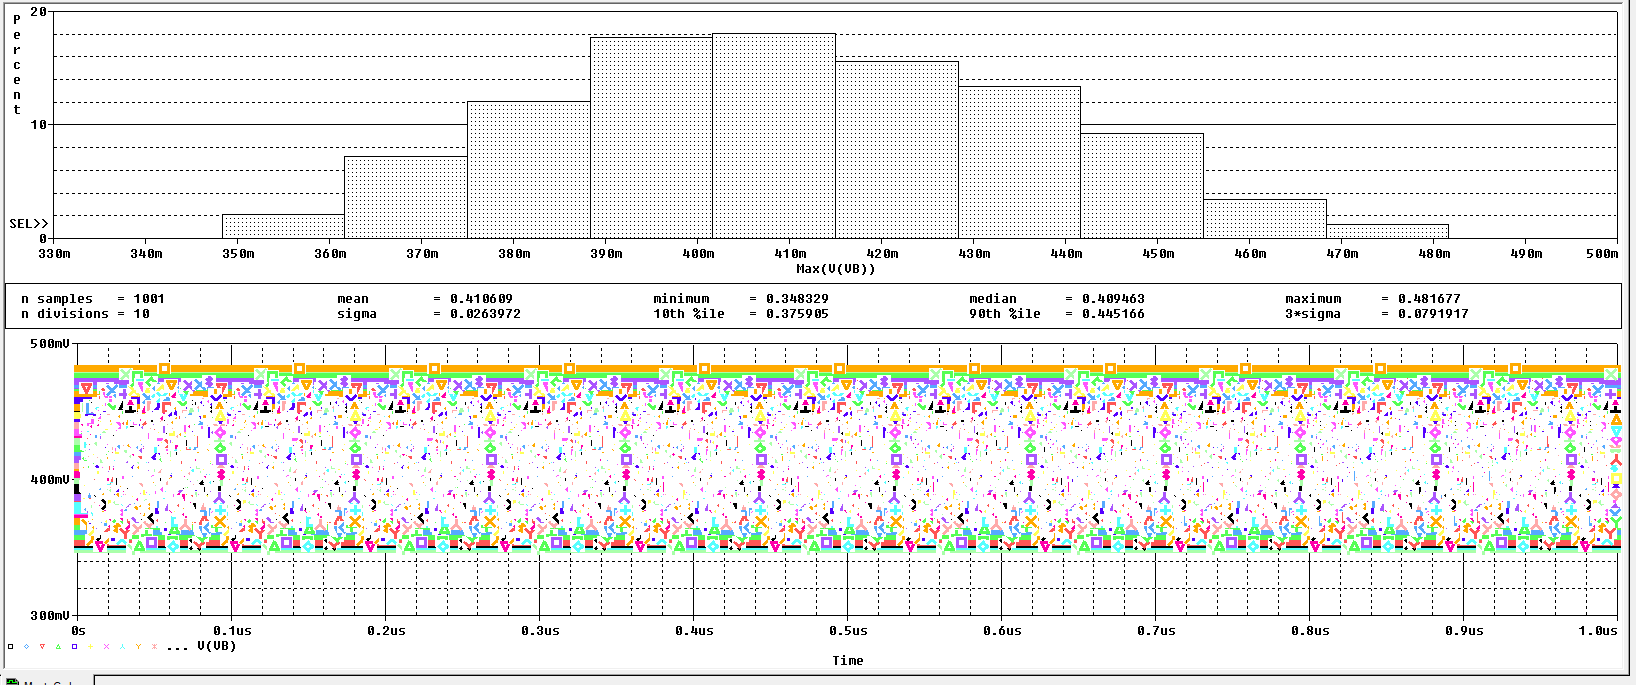
\includegraphics[width=\textwidth]{simulation}
	\caption{Monte Carlo of Circuit 1. }
	\label{Fig:Circuit1MonteCarlo}
\end{figure}

\section{Hardware Experiment: Results and Discussion}
This section of the report should present what was done in hardware.  A reader should be able to recreate an experiment from the detail present.  One section discusses the equipment used in the experiment. The remaining sections discuss the results for each circuit.
\subsection{Equipment Used in the Laboratory}
Write a short paragraph to detail the equipment used in the laboratory, and specific model numbers. Ideally, you should create a table of the equipment which should be referred to in text (See Table \ref{Table:Equipment} as an example).  The room location where the experiment was performed should be included.  Note that this should be a part of all Tech Memos, as it is an essential piece for other users to replicate your experiment.  \textbf{As you will be likely using the same equipment throughout the term, once the text/tables are established, you may reuse the information with the permission of your instructor/TA.}		
	\begin{table}[h!]
		\centering
		\caption{Equipment/Software required for Lab 1.}
		\label{Table:Equipment}
		%\begin{tabular}{llllll}
		\begin{tabular}{|c||c|c|c|c|}
			\hline
			Item & Tool & Room      \\
			\hline
			Simulation & OrCAD Capture CIS & All Open EE Labs   \\	 
			\hline 
			DC Power Supply&  Agilent E3630A  & 09-3170   \\	
			\hline  
			DC Power Supply & Agilent E3631A   & 09-3200 \\ 
			\hline 
			Multimeter & Agilent 34401A & 09-3170, 09-3200 \\
			\hline
			%				Oscilloscope & Textronix TDS2012C & 09-3200  \\
			%				\hline
			%				Oscilloscope & Agilent DSO 33120A & 09-3170  \\
			%				\hline
			%				
		\end{tabular}
	\end{table}

\subsection{Hardware Results/Discussion Circuit 1}	
  At least a paragraph should be included here to discuss the results. Some points to include are listed below:
\begin{itemize}
	\item Present the nodal voltages measured in Table \ref{Table:ResultsCircuit1}.
		\begin{table}[h!]
			\centering
			\caption{Experimental nodal voltages for Circuit 1.}
			\label{Table:ResultsCircuit1}
			%\begin{tabular}{llllll}
			\begin{tabular}{|c||c|c|c|}
				\hline
			Node & Voltage (\si{\volt}) & Percent Error With PSPICE \\
			\hline
			Supply & 5.002 &\\	 
			\hline 
			Node A & 2.708 &\\	 
			\hline
			Node B & 0.405 &\\	 
			\hline			
			\end{tabular}
		\end{table}
	\item Present the differential voltages measured in Table \ref{Table:DerivedResultsCircuit1}.  %Use Ohm's law as we did in the laboratory to complete the table.
			\begin{table}[h!]
				\centering
				\caption{Differential voltages and measured resistances for Circuit 1.}
				\label{Table:DerivedResultsCircuit1}
				%\begin{tabular}{llllll}
				\begin{tabular}{|c||c|c|c|c|c|}
					\hline
					Element & Component & Measured & Voltage  \\
					& Value & Resistance (\si{\ohm}) & (\si{\volt})     \\
				
					\hline
					Supply & 5~\si{\volt} & N/A & 5.002 \\	 
					\hline 
					$R_1$ & 5600~\si{\ohm} & 5560 & 2.292 \\	 
					\hline
					$R_2$ & 5600~\si{\ohm} & 5576 & 2.303 \\
					\hline
					$R_L$ & 1000~\si{\ohm} & 1005 & 0.405 \\
					\hline
				\end{tabular}
			\end{table}
	\item Kirchhoff's Voltage Law (sum of all voltages around a closed loop=0) is satisfied.   Provide a simple calculation to back this up.
%	\item Power conservation (sum of all powers around a closed loop = 0) is satisfied.
	\item Compare the measured result to the PSPICE for the \textbf{nodal voltages} reported in Table \ref{Table:ResultsCircuit1}. Perform an error analysis and report the data in the table.
\end{itemize}

%\subsection{Hardware Results/Discsussion Circuit 2}	
% At least a paragraph should be included here to discuss the results. Some points to include are listed below:
%\begin{itemize}
%	\item Present the nodal voltages measured in Table \ref{Table:ResultsCircuit2}.
%	\begin{table}[h!]
%		\centering
%		\caption{Experimental nodal voltages for Circuit 2.}
%		\label{Table:ResultsCircuit2}
%		%\begin{tabular}{llllll}
%		\begin{tabular}{|c||c|c|c|}
%			\hline
%			Node & Voltage (\si{\volt}) & Percent Error (Hand Calc.) & Percent Error (PSPICE) \\
%			\hline
%			Supply & & &\\	 
%			\hline 
%			Node A &  & &\\	 
%			\hline
%			Node B &  &  &\\	 
%			\hline				
%		\end{tabular}
%	\end{table}
%	
%	\item Present the differential voltages measured in Table \ref{Table:DerivedResultsCircuit2}.  Use Ohm's law as we did in the laboratory to complete the table.
%			\begin{table}[h!]
%				\centering
%				\caption{Derived Results for Circuit 2.}
%				\label{Table:DerivedResultsCircuit2}
%				%\begin{tabular}{llllll}
%				\begin{tabular}{|c||c|c|c|c|c|}
%					\hline
%					Element & Component & Measured & Voltage & Current & Power \\
%					& Value & Resistance (\si{\ohm}) & (\si{\volt}) & (\si{\ampere}) &  
%					(\si{\watt})    \\
%					\hline
%					Supply & 5~\si{\volt} & N/A & & &\\	 
%					\hline 
%					$R_1$ & 1000~\si{\ohm} & & & &\\	 
%					\hline
%					$R_2$ & 1000~\si{\ohm}& & & &\\	 
%					\hline
%					$R_L$ & 1000~\si{\ohm} & & & &\\	 
%					\hline
%					$R_{L2}$ & 180~\si{\ohm} & & & &\\	 
%					\hline				
%				\end{tabular}
%			\end{table}
%\end{itemize}
%For this circuit, in your report you should demonstrate: 
%\begin{itemize}
%	\item Kirchhoff's Voltage Law (sum of all voltages around a closed loop=0) is satisfied.   Do this for all closed loops in the circuit.  Provide a simple calculation to back this up.
%	\item Power conservation (sum of all powers around a closed loop = 0) is satisfied. Do this for all closed loops in the circuit.
%	\item Kirchhoff's Current Law (sum of currents entering a node is equal to 0) is satisfied. Show that current division can be used to explain the splitting of currents between $R_L$ and $R_{L2}$.
%	\item Compare the measured result to the PSPICE and theoretical calculations for the \textbf{nodal voltages} reported in Table \ref{Table:ResultsCircuit2}. Perform an error analysis and report the data in the table.
%\end{itemize}
	
	\section{Conclusion}
	Provide a 1 paragraph summary of the laboratory experiment.  What were the major conclusions for each circuit topology?  Also did the theory agree with the experiment?  The conclusion is a revised version of the abstract.
	
	\section{Acknowledgments}
	Acknowledge \textbf{any} source of help received in the experiment/writing the report.  This should certainly include your lab partner/teaching assistant/instructor.  It may also include other classmates/study partners. State briefly what the nature of the help was.
	
	\textbf{Your report should include references to appropriate pages in the text, as well as any other sources, websites/etc. consulted in the preparation of the report.}
\begin{thebibliography}{9}
	\bibitem{AlexanderSadiku}
	C.K. Alexander, and M.K.O. Sadiku,
	\emph{Fundamentals of Electric Circuits, 4th Edition},
	McGraw Hill, pp. xx-yy(EDIT), 2009.
	\bibitem{RommelLab}
	S. Rommel,
	\emph{EEEE 281 Lab 1 Lecture notes},
	slides xx-yy, Spring 2015.
\end{thebibliography}

\end{document}



